\documentclass[10pt,a4paper]{article}
\usepackage[utf8]{inputenc}
\usepackage{pgfplots}
\pgfplotsset{compat=1.16}
\usepackage{tikz}
\usetikzlibrary{automata,topaths,arrows,shapes}
\usetikzlibrary{backgrounds}
\usepackage{xcolor}
\usepackage{amsmath}
\usepackage{amssymb}

\begin{document}

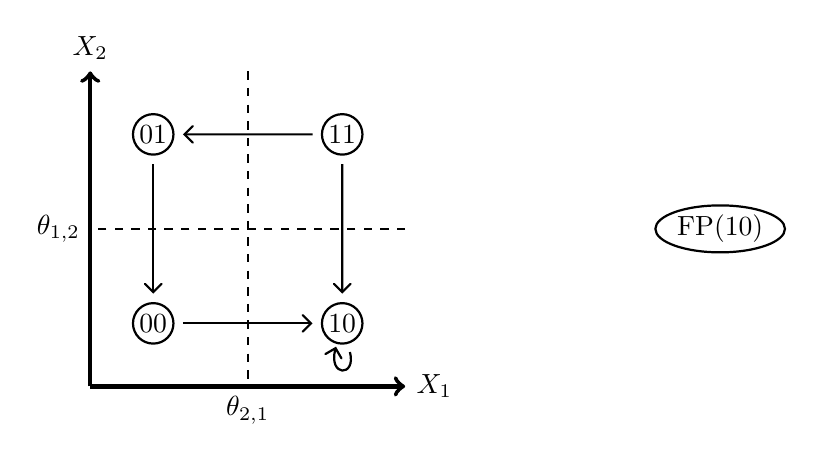
\begin{tikzpicture}[main node/.style={circle, draw, thick, inner sep=1pt, minimum size=0pt},scale=0.8]
\draw[dashed, thick] (5,2.5)--(0,2.5) node [left]{$\theta_{1,2}$};
\draw[dashed, thick] (2.5,5)--(2.5,0) node [below]{$\theta_{2,1}$};
\draw[->,ultra thick] (0,0)--(5,0) node[right]{$X_1$};
\draw[->,ultra thick] (0,0)--(0,5) node[above]{$X_2$};

\node[main node] (n1) at (1,1) {00};
\node[main node] (n2) at (1 , 4){01};
\node[main node] (n3) at (4,4) {11};
\node[main node] (n4) at (4 , 1){10};

\path[->,>=angle 90,thick]
(n1) edge[shorten <= 3pt, shorten >= 3pt] node[] {} (n4)
(n3) edge[shorten <= 3pt, shorten >= 3pt] node[] {} (n2)
(n3) edge[shorten <= 3pt, shorten >= 3pt] node[] {} (n4)
(n2) edge[shorten <= 3pt, shorten >= 3pt] node[] {} (n1)
(n4) edge[shorten <= 3pt, shorten >= 3pt, loop below] node[] {} (n4)
;

\node[main node,shape=ellipse] () at (10,2.5) {FP(10)};

\end{tikzpicture}

\end{document}